
En el código correspondiente del algoritmo de control \textit{Control Algorithm}~\cref{lst:Looper} el aspecto más relevante se encuentra en el cálculo de la variable controlada.
Para ello Se hace uso del Encoder; dentro del Dominio del controlador automático se ha desarrollado un modelo que lo representa.
El \textit{Encoder}~\cref{lst:Encoder} es una interfaz que actúa como puerto de salida hacia la implementación.
Define función de observación que llamaremos \textit{watchdog} de las lectura de dichos pines y una función a la que llamaremos para obtener la posición en el momento que deseemos, \textit{getPosition}.
También atañe al dominio saber que hay que restablecer los parámetros del encoder cuando se requiera y que hay que desactivar el hardware cuando se deje de utilizar para que no haya inconsistencias a la hora de volver a ejecutar el programa.
Para ello dispone de las otras funciones de la interfaz.

El adaptador\textit{Encoder Model}~\cref{lst:EncoderAdapter} hace uso de una librería en Go para Raspberry que permite la interacción con los pines de lectura con los que está conectado el encoder y realiza las operaciones pertinentes para obtener la posición.
El dispositivo particular en el que se va a ejecutar la lógica de control, el encoder físicamente conectado y todos los detalles finales del hardware no son más que un detalle de implementación secundario como lo es una base de datos.
El punto de más relevancia se encuentra enmarcado en rojo en el~\cref{lst:EncoderAdapter}.
Cuando se ejecuta la función de \textit{watchdog} se ponen en marcha dos \textit{gorutines}; una para vigilar cada lectura de los dos pines del Encoder.

Se queda en un bucle infinito la primera sentencia de dicho bucle es quedarse bloqueado hasta que haya un cambio en el pin de lectura, ya sea de 0 a 1 o de 1 a 0.
Si esto ocurre lo primero que hace es bloquear todas las demás \textit{gorutines}, porque va a hacer cambios en memoria de forma atómica, escribe la información de dicha lectura en un array de lecturas y desbloquea las \textit{gorutines}, se termina y vuelve a esperar.
Independientemente, el watchdog, una vez lanzadas las \textit{gorutines} de lectura se queda en bucle infinito que lo que hace es bloquear las \textit{gorutines}.
Extraer un elemento del array de lecturas y procesarlo.

Tal y como están diseñadas la \textit{gorutines}, se van encolando y esperan su momento en la CPU para ejecutarse.
Si hay bloqueos también esperan su turno.
De esta forma, aunque el procesamiento de una lectura fuera bloqueado por el sistema operativo, se irían encolando las \textit{gorutines} a la espera de poder añadirse en el array de lecturas, pero no se perderían.
De esta forma se consigue leer exactamente los 360 pulsos por vuelta del encoder sin perder ninguno.


\phantom{blank}
\vspace{5mm}
\hrule
\begin{lstlisting}[language=Go,caption={ControlAlgoritm.go},breaklines=true,label={lst:ControlAlgoritm}]
package Entity

type ControlAlgorithm interface {
    SetGoal(goal float64)
    SetP(p float64)
    SetI(i float64)
    SetD(d float64)
    SetSampleTime(d float64)
    GetIntegralTerm() float64
    Calculate(currentValue float64) float64
}

type controlAlgorithm struct {
    goal         float64
    P            float64
    I            float64
    D            float64
    integralTerm float64
    sampleTime   float64
    currentValue float64
    currentError float64
    pastError    float64
}

func NewControlAlgorithm() ControlAlgorithm {
    return &controlAlgorithm{}
}

func (ca *controlAlgorithm) SetGoal(goal float64) {
    ca.goal = goal
}

func (ca *controlAlgorithm) SetP(p float64) {
    ca.P = p
}

func (ca *controlAlgorithm) SetI(i float64) {
    ca.I = i
}

func (ca *controlAlgorithm) SetD(d float64) {
    ca.D = d
}

func (ca *controlAlgorithm) GetIntegralTerm() float64 {
    return ca.integralTerm
}

func (ca *controlAlgorithm) SetSampleTime(st float64) {
    ca.sampleTime = st
}

func (ca *controlAlgorithm) Calculate(currentValue float64) float64 {
    ca.currentValue = currentValue
    ca.currentError = ca.goal - ca.currentValue
    proportionalTerm := ca.P * ca.currentError
    ca.integralTerm = ca.integralTerm + ca.currentError*ca.sampleTime
    derivativeTerm := ca.D * (ca.currentError - ca.pastError) / ca.sampleTime
    ca.pastError = ca.currentError
    return proportionalTerm + ca.I*ca.integralTerm + derivativeTerm

}

\end{lstlisting}
\hrule
Dentro del Dominio del controlador tendremos Un modelo de lo que significa para nosotros un encoder. Podemos ver en la figura \ref{fig:EncoderInterface} que es una interfaz que actua como puerto de salida hacia la implementación, el adaptador que contemplará el uso de una librería en golang para raspberry que permita la interacción de los pines de lectura con los que está conectado el encoder y realice las operaciones pertinentes para obtener la posición. Todo esto no es responsabilidad del Dominio. No nos atañe el dispositivo en el que se va a ejecutar la lógica de control a partir de este encoder. Simplemente nos interesa que tenga una función de observación que llamaremos \textit{watchdog} de las lectura de dichos pines y una función a la que llamaremos para obtener la posición en el momento que deseemos saberlo \textit{getPosition} También atañe al dominio saber que hay que resetear los parámetros del encoder cuando interese y que hay que desactivar el hardware cuando se deje de utilizar para que no haya inconsistencias a la hora de volver a ejecutar el programa.


\begin{figure}[H]
    \centering
    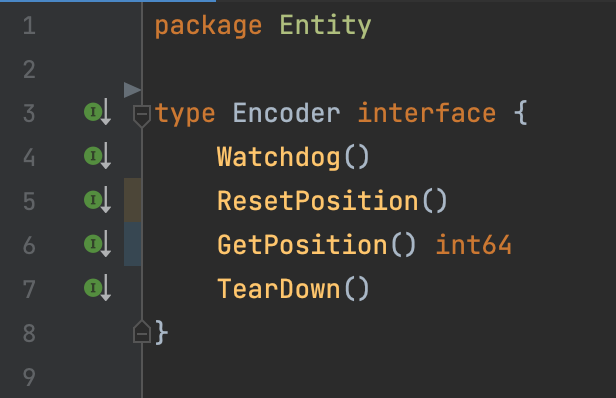
\includegraphics[height=0.2\textheight]{./part/Ejecucion/Seguimiento/Encoder/img/EncoderInterface}
    \caption{Encoder.go}\label{fig:EncoderInterface}
\end{figure}

Pasando a la implementación el punto de más relevancia se encuentra remarcado en rojo en la figura \ref{fig:EncoderAdapter} donde podemos ver que cuando se ejecuta la función de \textit{watchdog} se ponen en marcha dos gorutines; una para vigilar cada lectura de los dos pines del Encoder.

Se queda en un bucle infinito la primera sentencia de dicho bucle es quedarse bloqueado hasta que haya un cambio en el pin de lectura, ya sea de 0 a 1 o de 1 a 0. Si esto ocurre lo primero que hace es bloquear todas las demas gorutines porque va a hacer cambios en memoria de forma atómica, escribe la información de dicha lectura en un array de lecturas y desbloquea las gorutines, se termina y vuelve a esperar.

Independientemente, el watchdog, una vez lanzadas las gorutines de lectura se queda en bucle infinito que lo que hace es bloquear las gorutinas. Extraer un elemento del array de lecturas y procesarlo.

Tal y como están diseñadas la gorutines, se van encolando y esperan su momento en la CPU para ejecutarse. si hay bloqueos también esperan su turno. De esta forma supongamos que el procesado de una lectura tardara más de la cuenta. Se irían encolando las gorutines a la espera de poder añadirse en el array de lecturas, pero no se perderían. De esta forma Se consigue leer exactamente los 360 pulsos por vuelta del encoder sin perder ninguno.

\begin{figure}[H]
    \centering
    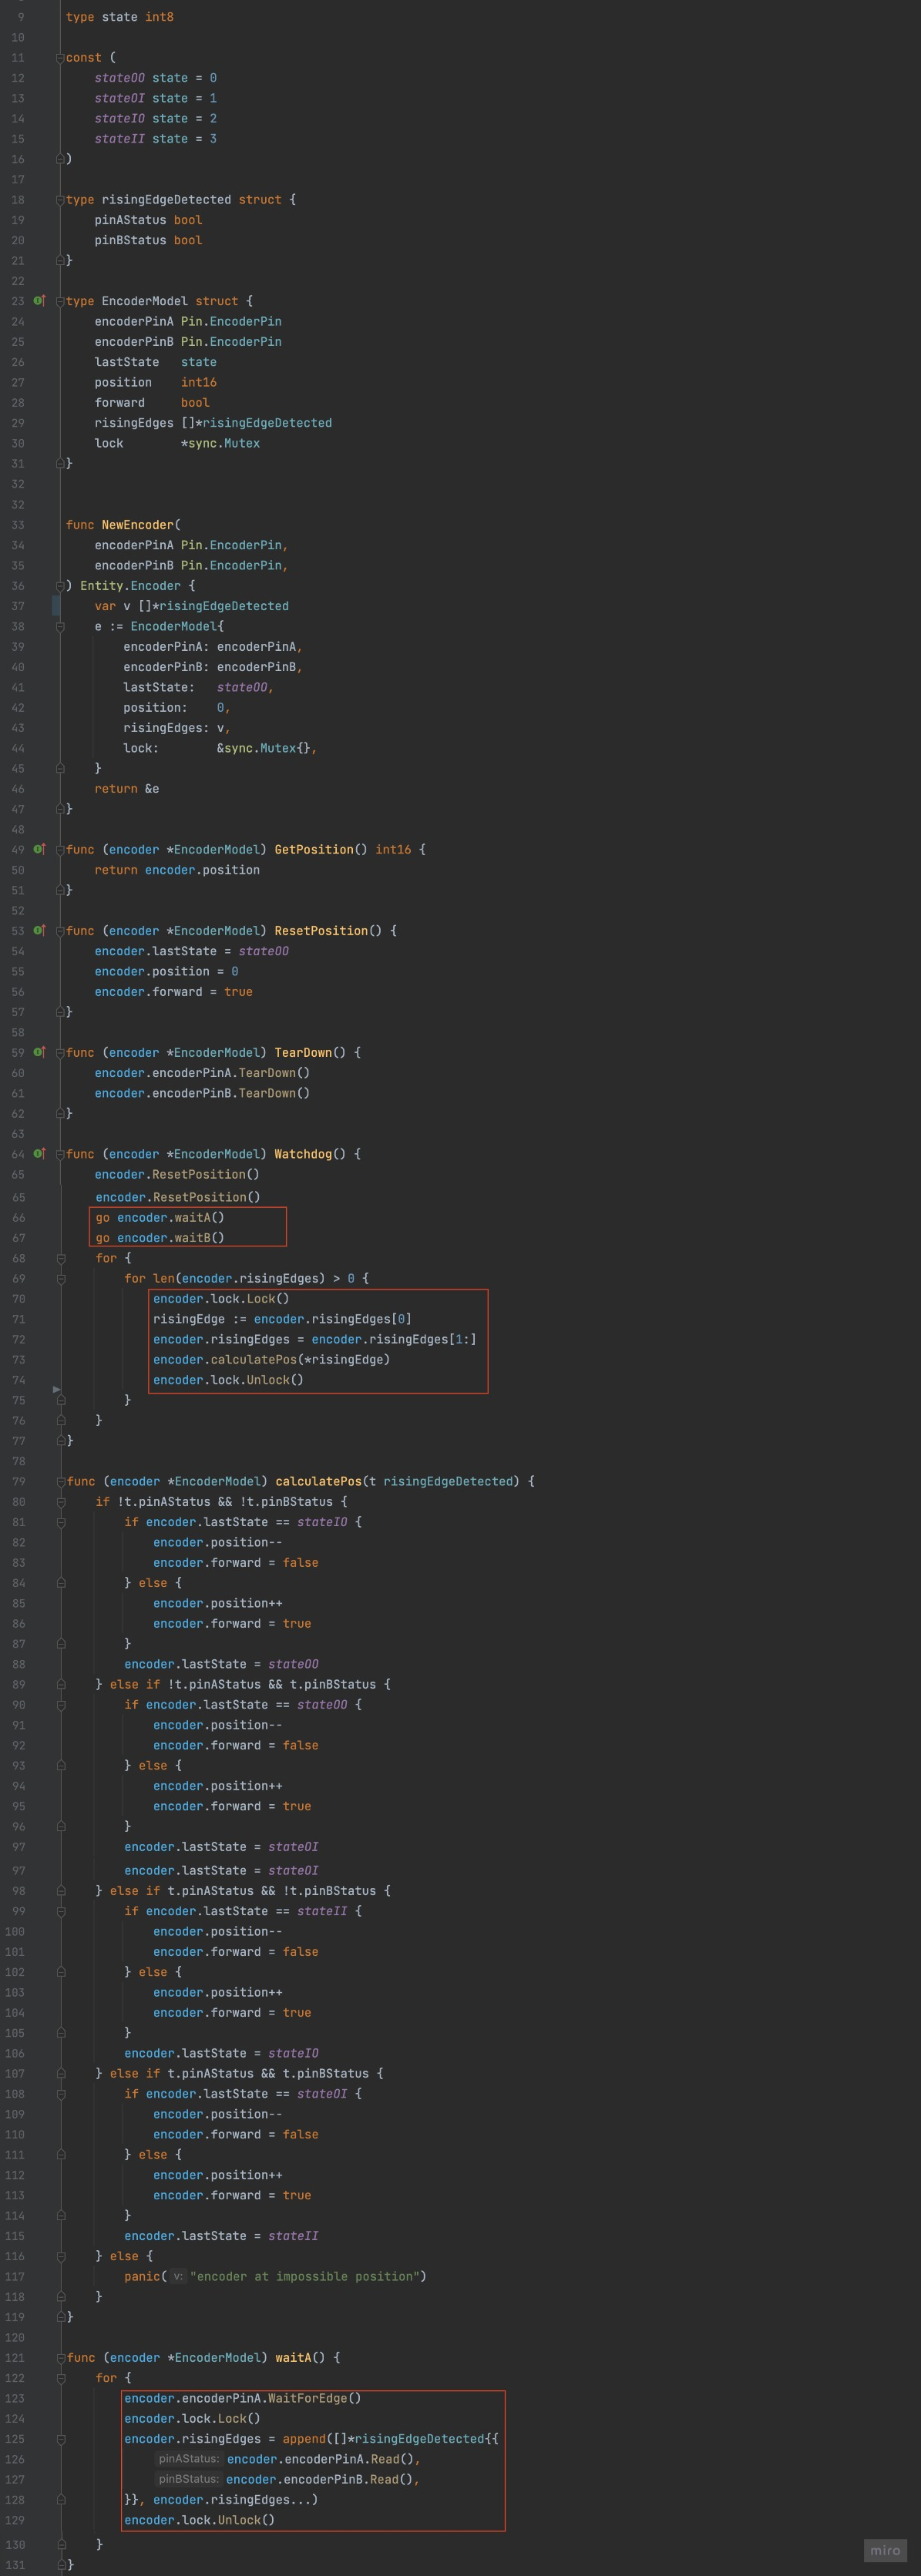
\includegraphics[height=0.95\textheight]{./part/Ejecucion/Seguimiento/Encoder/img/PFM - Encoder}
    \caption{EncoderAdapter.go}\label{fig:EncoderAdapter}
\end{figure}

\phantom{blank}
\vspace{5mm}
\hrule
\begin{lstlisting}[language=Go,caption={EncoderAdapter.go},breaklines=true,label={lst:EncoderAdapter}]
package Model

import (
	"github.com/Enrikerf/pfm/commandExecutor/app/Domain/Entity"
	"github.com/Enrikerf/pfm/commandExecutor/app/Domain/Entity/Pin"
	"sync"
)

type state int8

const (
	stateOO state = 0
	stateOI state = 1
	stateIO state = 2
	stateII state = 3
)

type risingEdgeDetected struct {
	pinAStatus bool
	pinBStatus bool
}

type EncoderModel struct {
	encoderPinA Pin.EncoderPin
	encoderPinB Pin.EncoderPin
	lastState   state
	position    int64
	forward     bool
	risingEdges []*risingEdgeDetected
	lock        *sync.Mutex
}

func NewEncoder(
	encoderPinA Pin.EncoderPin,
	encoderPinB Pin.EncoderPin,
) Entity.Encoder {
	v := []*risingEdgeDetected{}
	e := EncoderModel{
		encoderPinA: encoderPinA,
		encoderPinB: encoderPinB,
		lastState:   stateOO,
		position:    0,
		risingEdges: v,
		lock:        &sync.Mutex{},
	}
	return &e
}

func (encoder *EncoderModel) GetPosition() int64 {
	return encoder.position
}

func (encoder *EncoderModel) ResetPosition() {
	encoder.lastState = stateOO
	encoder.position = 0
	encoder.forward = true
}

func (encoder *EncoderModel) TearDown() {
	encoder.encoderPinA.TearDown()
	encoder.encoderPinB.TearDown()
}

func (encoder *EncoderModel) Watchdog() {
	encoder.ResetPosition()
	go encoder.waitA()
	go encoder.waitB()
	for {
		for len(encoder.risingEdges) > 0 {
		<@\textcolor{red}{--Atomic action--}@>
			encoder.lock.Lock()
			risingEdge := encoder.risingEdges[0]
			encoder.risingEdges = encoder.risingEdges[1:]
			encoder.calculatePos(*risingEdge)
			encoder.lock.Unlock()
		<@\textcolor{red}{-----}@>
		}
	}
}

func (encoder *EncoderModel) calculatePos(t risingEdgeDetected) {
	if !t.pinAStatus && !t.pinBStatus {
		if encoder.lastState == stateIO {
			encoder.position--
			encoder.forward = false
		} else {
			encoder.position++
			encoder.forward = true
		}
		encoder.lastState = stateOO
	} else if !t.pinAStatus && t.pinBStatus {
		if encoder.lastState == stateOO {
			encoder.position--
			encoder.forward = false
		} else {
			encoder.position++
			encoder.forward = true
		}
		encoder.lastState = stateOI
	} else if t.pinAStatus && !t.pinBStatus {
		if encoder.lastState == stateII {
			encoder.position--
			encoder.forward = false
		} else {
			encoder.position++
			encoder.forward = true
		}
		encoder.lastState = stateIO
	} else if t.pinAStatus && t.pinBStatus {
		if encoder.lastState == stateOI {
			encoder.position--
			encoder.forward = false
		} else {
			encoder.position++
			encoder.forward = true
		}
		encoder.lastState = stateII
	} else {
		panic("encoder at impossible position")
	}
}

func (encoder *EncoderModel) waitA() {
	for {
		encoder.encoderPinA.WaitForEdge()
		encoder.lock.Lock()
		encoder.risingEdges = append([]*risingEdgeDetected{{
			encoder.encoderPinA.Read(),
			encoder.encoderPinB.Read(),
		}}, encoder.risingEdges...)
		encoder.lock.Unlock()
	}
}

func (encoder *EncoderModel) waitB() {
	for {
		encoder.encoderPinB.WaitForEdge()
		encoder.lock.Lock()
		encoder.risingEdges = append([]*risingEdgeDetected{{
			encoder.encoderPinA.Read(),
			encoder.encoderPinB.Read(),
		}}, encoder.risingEdges...)
		encoder.lock.Unlock()
	}
}

\end{lstlisting}
\hrule